% LaTeX file for a 1 page document
\documentclass[12pt]{article}
\usepackage{graphicx}
\usepackage{wrapfig}
\usepackage{fullpage}
\usepackage{url}
\usepackage{listings}

\lstdefinestyle{basic}{showstringspaces=false,columns=fullflexible,language=Java,
escapechar=@,xleftmargin=1pc,%
%basicstyle=\small\bfseries\itshape,%
%keywordstyle=\underbar,
mathescape=true,%
lineskip=-1pt,%
keepspaces=true,%
%basicstyle=\small\sffamily,%
basicstyle=\footnotesize\ttfamily,%
commentstyle=\mdseries\rmfamily,%
morekeywords={class,object,with,fun,new,end,int,bool,string},%
deletekeywords={error,apply,values,and,equal,eq},%
moredelim=**[is][\color{red}]{`}{`}
}
\lstset{style=basic}

\title{C343 Project - Routing Wires on a Chip}
\date{}

\begin{document}
\maketitle

\section{Project Description}

In this project you will implement a Java program that places wires
on a computer chip. For purposes of this project, a computer chip will
be abstractly represented as a grid of vertices, where each vertex is
connected to the four neighboring vertices (in the directions north,
south, east, and west). To complicate matters, parts of the chip are
already allocated for other uses and may not be used for running
wires. These already-in-use parts are called obstacles. Each obstacle
is a rectangular region of the grid. You will be given a list of pairs
of coordinates and your task is to connect each pair with a wire.  A
coordinate is a pair of integers, with the first being the horizontal
distance from the left edge of the grid, and the second being the
vertical distance from the top edge of the grid.  A wire is a list of
grid points. Wires may not cross one another.  In addition to
connecting all the pairs, your goal is to minimize the aggregate
lengths of all the wires and to minimize the execution time of your
program.

The format of the input file is described as follows.  The first line
is the height of the grid, given as an integer.  The second line is
the width of the grid, also given as an integer.  The third line is
the number of obstacles $o$.  The next $o$ lines are the obstacles.
Each line has four integers, separated by spaces. The first two
integers give the upper left coordinate of the obstacle and the second
two integers give the lower right coordinate of the obstacle.  After
the obstacles, there is a line that gives the number of pairs that
need to be connected. The remaining lines in the file are pairs of
space-separated coordinates, where each coordinate is a pair of
space-separated integers.

We have given you the code that reads the input file and creates the grid
with obstacles laid out and the source and destination points specified.
%% For example, the grid generated for the file \texttt{gen\_chip\_1\_1.in} is
%% shown in Figure~\ref{fig:board}. 
The obstacles are marked with grid cells with value $-1$. The start
and end points of a wire/path are marked with a number assigned to
that path. All the other cells contain the value $0$.

Your function \lstinline{findPaths} in the \lstinline{Routing} class
should use this grid to connect a source and a destination with a
path. You should mark the grid once a path has been found for a pair
of points, thus preventing overlapping of paths. Also all the points
that lie on an obstacle should be avoided. The
\lstinline{checkCorrectness} function in the \lstinline{Drive} class
checks for these conditions to verify the correctness of your
solution.

%% \begin{figure}
%% 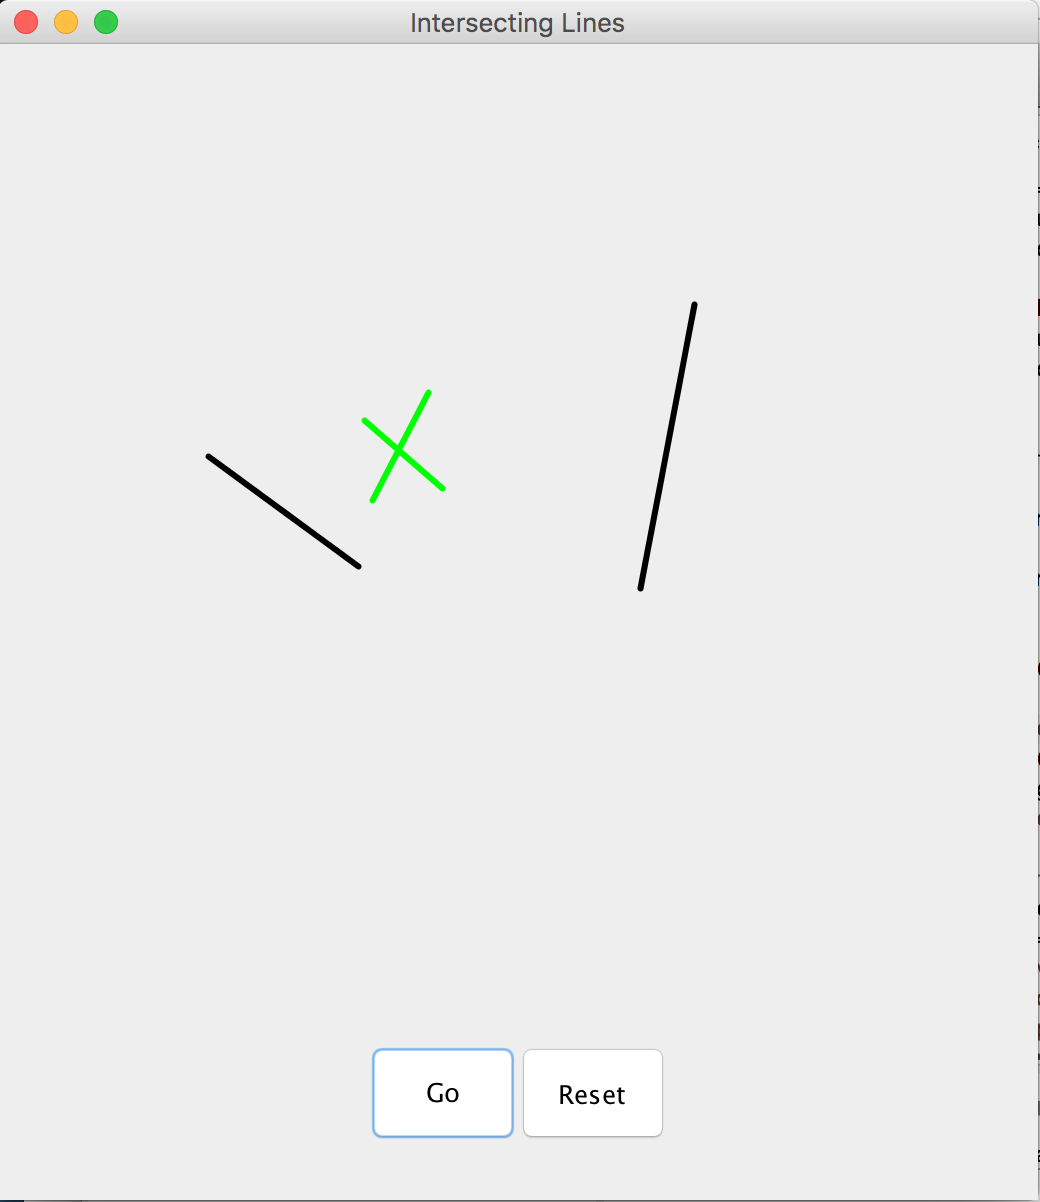
\includegraphics[scale=0.35]{board.png}
%% \label{fig:board}
%% \end{figure}

Note that a path can have the same source and destination points.

\section{Your Task}

We need you to implement the following method:
\begin{enumerate}
\item \lstinline{findPaths} - Takes the board and the points to be
  connected as arguments and returns a list of paths. The board
  represents the entire chip. Each path represents the wire used to
  connect components represented by points. Each path connects a pair
  of points in the points array; avoiding obstacles and other paths
  while minimizing the total path length required to connect all
  points. If two points cannot be connected, then the path should be
  null.
\end{enumerate}

Think of a simple way to minimize the path length. You can use the
grid to mark the points that lie on a path.  You might want to use
auxiliary data structures to keep track of the intermediate points
that lie on the path.

After finding a correct solution, you can look for heuristics to
reduce the aggregate length further.

\section{Running Your Code}

To run, execute \texttt{java -cg ./src Driver test \textit{chipfile}}
where \textit{chipfile} is any of the \textit{.in} files provided in
the \texttt{Inputs} directory. The driver will run your
\lstinline{findPaths} function. To run all of the tests in the
\texttt{Inputs} directory, execute \texttt{java -cg ./src Driver
  batch\_test}.

\section{Deliverables}

Your repository should contain all the files from the zip.  We will be
looking at the following while grading your assignment:
\begin{itemize}
\item \texttt{Routing.java} - containing your solution
\item Describe your solution in \texttt{README.md}.
\item Hours - record the number of hours you spent on writing and
  debuging your code. Put your answers in the \texttt{README.md}.
\end{itemize}


\end{document}
